\documentclass[11pt]{article}
\usepackage{fullpage}
\usepackage{amsmath}
\usepackage{amssymb}
\usepackage{graphicx}
\usepackage{color}
\usepackage{float}
\usepackage{caption}
\usepackage{placeins}

\renewcommand\baselinestretch{1.5}
\newcommand{\Pose}{{\cal P}}
\newcommand{\A}{{\cal A}} 
\newcommand{\X}{\mathbf{X}} 
\newcommand{\symb}{\Sigma}
\newcommand{\actP}{P^{\A}}
\newcommand{\B}{\cal B}
\newcommand{\Xrm}{\X^{\Am}_{-r}}
\newcommand{\Am}{\A_{m}} 
\newcommand{\Real}{\mathbb{R}}
\newcommand{\gcomp}{comp(\mathbf{g}^{\Am})}

\begin{document}

\title{Jeroen's model}
\maketitle

\section{Notation}

\begin{itemize}

\item $\symb$: partially-ordered list of symbols (types).

\item $\symb_i$: ith symbol in partial ordering.

\item $T$: number of symbols in grammar.

\item $\Pose$: pose space.

\item ${\B} = (b_1,\ldots,b_N)$: set of bricks.

\item $\Pose(b) \in \Pose$: set of poses associated with brick $b$.

\item $\A = (a_1,\ldots,a_M)$, $\A \subseteq {\B}$: set of active bricks.

\item $\Am = (a_1,\ldots,a_m)$, $m \leq M$ $\Am \subseteq {\A}$: subset of active bricks.

\item $t(b)$: type of brick $b$.

\item $\#(C)$: the cardinality (size) of some set $C$. \emph{E.g.} $\#(\A)=M$.

\item ${\cal R}$: set of production rules of the form
$A \rightarrow B_1,\ldots,B_k$ with $r = A,B_1,\ldots,B_k \in \Sigma$. ${\cal R}$ is acyclic.

\item $n(r)$: number of slots/children associated with rule $r \in {\cal R}$

%\item ${\cal R}(b)$: rules with $t(b) \in \B$ in the LHS.
\item $c(b)$: the set of production rules with $t(b)$ in the LHS.

%\item $p_b$: distribution over ${\cal R}(b)$.
\item $\vec{\theta}_b \in \mathbb{R}^{\#(c(b))}$: distribution over rules with  $t(b) \in \B$ in the LHS.

%\item $p_{r,n}(x_i|x)$, $r \in {\cal R}$, $x,x_i \in {\cal P}$, $n \in [1...n(r)]$: 
conditional probability density over pose for $B_i$ given pose for $A$ for this rule and slot.

\item $s_b \in \{0,1\}$: on/off state of brick $b$.

\item $r_b \in {\cal R}(t(b))$: rule used by brick $b$.

\item $\mathbf{g_b} \in ( {\B} \cup \perp )^{c(b)}$: array of pointers, where each element can either point to a brick, or null (no child).

\item $\mathbf{g}_b^{\Am} \in ( {\Am} \cup \emptyset )^{c(b)}$: array of pointers, where each element can either point to a brick in the active set defined by $\Am$, or blank (child not yet specified) denoted by $\emptyset$. Note that blank is \textbf{different} than null (no child) in that blank means ``there could be a child in this slot, but we don't know if there is or which one yet'' while null (no child) means ``there definitely isn't a child in this slot''.

\item $\gcomp$: the elements of $\mathbf{g}^{\Am}$ for which $g_{b,k}^{\Am} == \emptyset$. Note: we use ``comp'' as the identifier for this concept since these are the slots that may receive a child in the future; these are the slots to be``completed''.

\item $V(b)$: ``before'' set of bricks, which we define as $V(b) = \{b' : t(b') < t(b) \}$ where $<$ means ``comes before in the partial ordering defined by $\symb$''.

\item $W(b)$: ``after'' set of bricks, which we define as $V(b) = \{b' : t(b') > t(b) \}$ where $>$ means ``comes after in the partial ordering defined by $\symb$''.

\item $\vec{\phi}_{b,k,r} \in \mathbb{R}^{\#(W(b))+1}$: distribution over bricks to which brick $b$'s $k-th$ slot may point if brick $b$ is using rule $r$. Note that brick $b$ may only point to bricks in its ``after'' set. Note that the $+1$ is present since a brick/slot may point to nothing, denoted by the symbol $\perp$. \emph{edit}: this is a bit sloppy. Each slot has a particular type, and only bricks of that type may go in this slot. The set of possibilities for each slot, in general, is a subset of the ``after'' set, and not the entire after set.

\item $q_b \in \Pose(b)$: pose for brick $b$. $q_b = \perp$ is a special ``nothing'' pose that does not contribute to image evidence.

\item $\vec{\pi} \in \Real^T$: vector of mixing coefficients for the templates of each type of brick.

\item $\X = \{ \mathbf{s}, \mathbf{r}, \mathbf{g}, \mathbf{q}\}$: collection of hidden variables of model.

\item $\Xrm = \{s_a, g_a, q_a\}, \forall a \in \Am$: collection of hidden variables of model, with rules removed, for the set of bricks in the active set.

\item $I$: the image.

\end{itemize}

\section{Model}

\begin{figure}[htbp]
\begin{center}
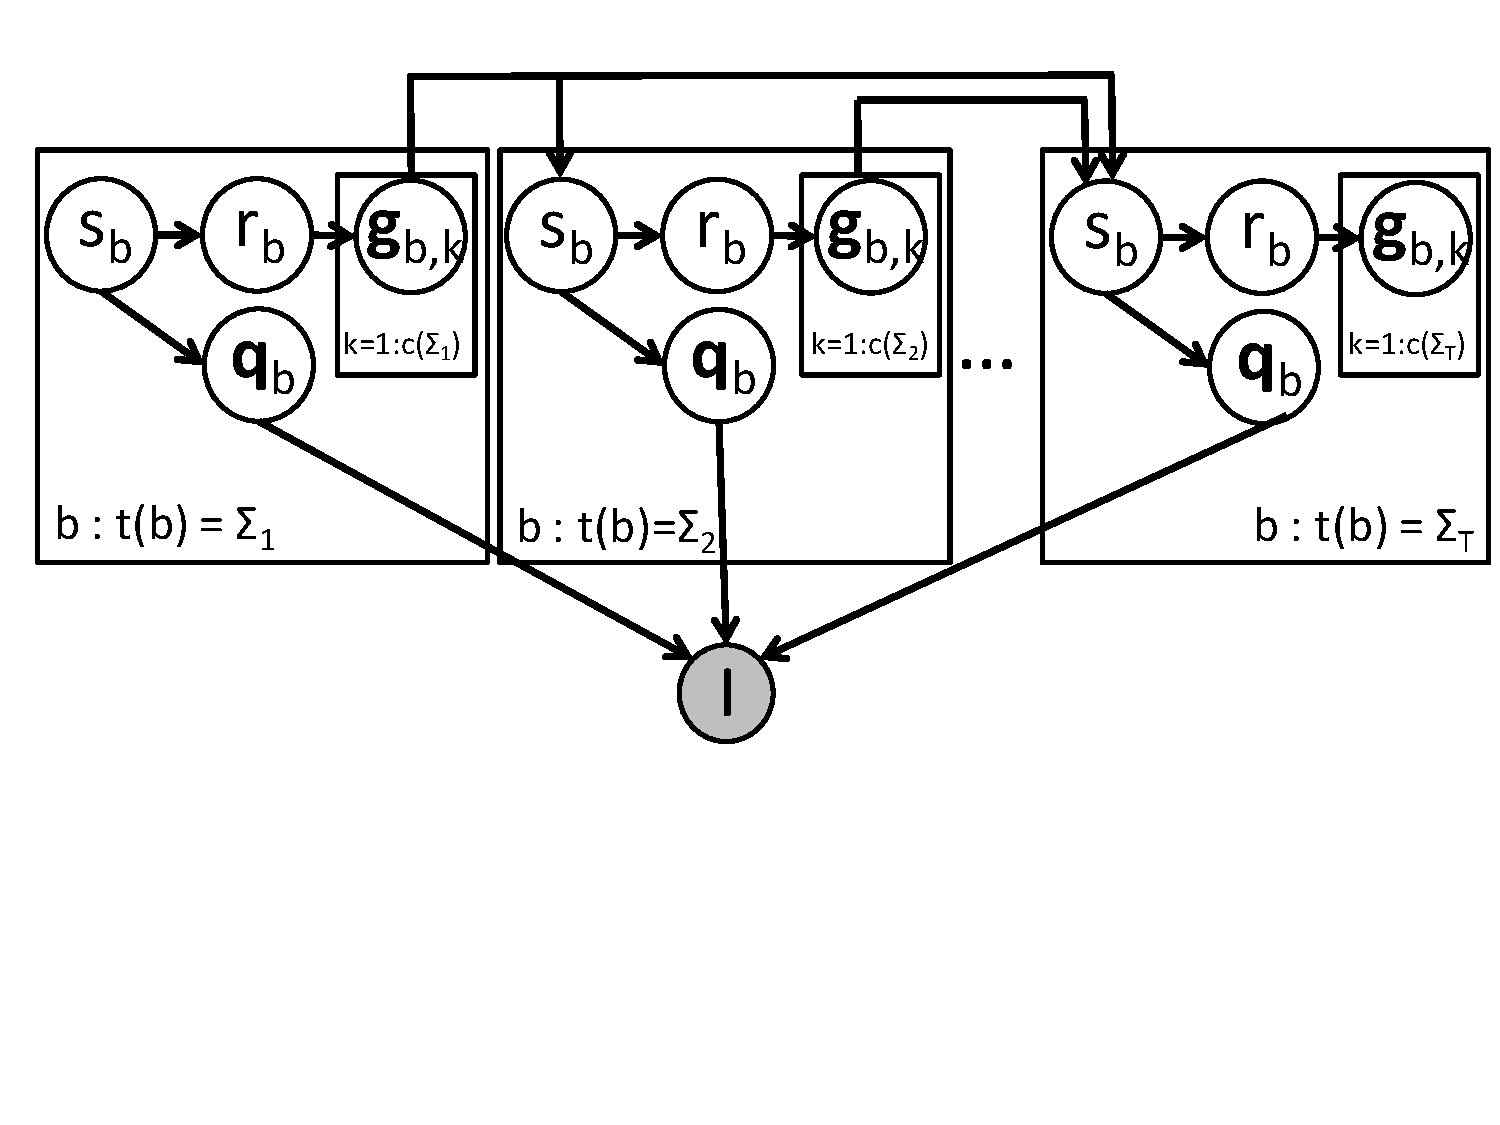
\includegraphics[width=\textwidth, trim=0cm 6cm 0cm 0cm]{gm.pdf}
\caption{Graphical model}
\label{gm}
\end{center}
\end{figure}

\FloatBarrier

The decomposition of the joint probability is given by the graphical model in Fig. \ref{gm} and by: \\

\begin{eqnarray}
P(\X, I) &=& \big({\displaystyle \prod_{b \in {\B}}} P(s_b \mid \mathbf{g}_{V(b)}) \big ) \\
& &\big( {\displaystyle \prod_{b \in {\B}}} P(r_b \mid s_b) {\displaystyle \prod_{k=1}^{c(b)}} P(g_{b,k} \mid r_b) \big) \nonumber \\
& &\big( {\displaystyle \prod_{b \in {\B}}} P(\mathbf{q_b} \mid s_b)\big) \nonumber \\
& & P(I \mid \mathbf{q}) \nonumber 
\end{eqnarray}
%
where we define the following pieces:
%
\begin{eqnarray}
P(s_b = 1 \mid \mathbf{g}_{V(b)}) &=&  \begin{cases} 1 \mbox{ if } \exists \{a,k\} \mbox{ s.t. } g_{a,k} = b \mbox{ , } g_{a,k} \in {g}_{V(b)} \\
\epsilon \mbox{ if } \nexists \{a,k\} \mbox{ s.t. } g_{a,k} = b \mbox{ , } g_{a,k} \in {g}_{V(b)} \end{cases} \\
P(r_b \mid s_b) &=& Discrete(\vec{\theta}_b) \\
P(g_{b,k} \mid r_b) &=& Discrete(\vec{\phi}_{b,k,r_b}) \\
P(\mathbf{q_b} = q \mid s_b)\big) &=& \begin{cases} \frac{1}{\#\Pose(b)} \mbox{ if } s_b = 1 \mbox{ and } q \neq \perp, q \in \Pose(b) \\
                                                   0 \mbox{ if } s_b = 1 \mbox{ and } q == \perp \\
                                                   0 \mbox{ if } s_b = 0 \mbox{ and } q \neq \perp \\
                                                   1 \mbox{ if } s_b = 0 \mbox{ and } q == \perp  \end{cases} \\
P(I \mid \mathbf{q}) &=& {\displaystyle \prod_{p}} P(I_p \mid \mathbf{q}) \\
P(I_p \mid \mathbf{q}) &\propto& {\displaystyle \sum_{b}} \pi_{t(b)}P(I_p \mid q_b) \delta(q_b \text{ overlaps with } p) \\
P(I_p \mid q_b) &=& \text{defn on where pixel p falls in template t(b) here, along with statement of prob. being Bernoulli distribution}.
\end{eqnarray}

where $\delta(\cdot)$ is an indicator variable.


\section*{Localization}

%For localization, we do not explicitly represent $\mathbf{r}$; instead we express the state configuration in terms of $\mathbf{g}_b^{\A}$ only, which implicitly specifies a set of compatible rules. Rather than selecting specific values for $\mathbf{r}$, we instead marginalize over the set of compatible rules defined by $\mathbf{g^{\A}}$ wherever  $\mathbf{r}$ is referred to.

We define localizations in terms of the components $\big({\displaystyle \prod_{b \in {\B}}} P(s_b \mid \mathbf{g}_{V(b)}) \big )$, $\big( {\displaystyle \prod_{b \in {\B}}} P(r_b \mid s_b) {\displaystyle \prod_{k=1}^{c(b)}} P(g_{b,k} \mid r_b) \big)$, $\big( {\displaystyle \prod_{b \in {\B}}} P(\mathbf{q_b} \mid s_b)\big)$, and $P(I \mid \mathbf{q})$ separately.

\begin{eqnarray}
\big({\displaystyle \prod_{b \in {\B}}} P(s_b \mid \mathbf{g}_{V(b)}) \big ) &\Rightarrow& \big({\displaystyle \prod_{a \in {\Am}}} P^{\Am}(s_a \mid \mathbf{g}^{\Am}_{V({b})}) \big )
\end{eqnarray}

where $\Rightarrow$ is used to mean ``localiizes to'', and we evaluate $P^{\Am}(s_a \mid \mathbf{g}^{\Am}_{V({b})})$ in a similar fashion to $P(s_b \mid \mathbf{g}_{V(b)})$ outlined above. We note that $P^{\Am}(s_a \mid \mathbf{g}^{\Am}_{V({b})}) \neq P(s_a \mid \mathbf{g}^{\Am}_{V({b})})$ since we do not perform the ``correct'' marginalizations.

Similarily, 

\begin{eqnarray}
\big( {\displaystyle \prod_{b \in {\B}}} P(r_b \mid s_b) {\displaystyle \prod_{k=1}^{c(b)}} P(g_{b,k} \mid r_b) \big) &\Rightarrow& \big( {\displaystyle \prod_{a \in \Am}} P(r_a \mid s_a) {\displaystyle \prod_{k=1}^{c(b)}} P^{\Am}(g_{a,k} \mid r_a) \big) \\
%
P^{\Am}(g_{a,k} \mid r_a) &=& \begin{cases} \label{actPg} 1-{\displaystyle \sum_{a' \in {\Am}}} P(g_{a,k} = a' \mid r_a) \mbox{ if } g_{a,k} == \emptyset \\
 P(g_{a,k} \mid r_a) \mbox{ , otherwise } \end{cases}
\end{eqnarray}
Note that the RHS of Eqn. (\ref{actPg}) is defined in terms of non-localized distributions, $P(g_{a,k} \mid r_a)$.

\begin{eqnarray}
\big( {\displaystyle \prod_{b \in {\B}}} P(\mathbf{q_b} \mid s_b)\big) \Rightarrow \big( {\displaystyle \prod_{a \in {\Am}}} P(\mathbf{q_a} \mid s_a)\big)
\end{eqnarray}
\begin{eqnarray}
P(I \mid \mathbf{q}) \Rightarrow P^{\Am}(I \mid \mathbf{q^{\Am}}) \label{Pim}
\end{eqnarray}

where we evaluate Eqn. \ref{Pim} in a similar fashion to $P(I \mid \mathbf{q})$. We note that $P^{\Am}(I \mid \mathbf{q^{\Am}}) \neq P(I \mid \mathbf{q^{\Am}})$ since we do not perform the correct marginalizations.

We define the overall localized distribution, $P^{\Am}(X^{\Am}$, I), in terms of the previously defined localization distributions:
\begin{eqnarray}
P^{\Am}(X^{\Am}, I)
&=& \big({\displaystyle \prod_{a \in {\Am}}} P^{\Am}(s_a \mid \mathbf{g}^{\Am}_{V({b})}) \big ) \label{eqn.localJoint}\\
& & \big( {\displaystyle \prod_{a \in {\Am}}} P(r_a \mid s_a) {\displaystyle \prod_{k=1}^{c(b)}} P^{\Am}(g_{a,k} \mid r_a) \big) \nonumber \\
& & {\displaystyle \prod_{a \in {\Am}}} P(\mathbf{q_a} \mid s_a)\big) \nonumber \\
& & P^{\Am}(I \mid \mathbf{q^{\Am}}) \nonumber
\end{eqnarray}

\section*{State representation}

Representing the configuration of an image for a \textbf{non-localized} model requires specifying $s_b$, $g_b$, $r_b$, $q_b$, $\forall b \in \B$. For a \textbf{localized} model, the same random variables could be used as the state representation. However, requiring specification of the $r_b$'s is unnecessary and too restrictive; we may not be able to well predict the rule a brick has used by examining the set of active bricks. This is especially true if the active set only contains one brick! Instead, we represent the state representation of the localized model by the random variables $\Xrm = \{s_a$, $g_a$, $q_a\}$, $\forall a \in \A$, and we marginalize over $r_a$ wherever it is used.

\section*{Inference}

Inference proceeds by iteratively adding one brick at a time to the active set. At any iteration, $m$, our goal is to maintain a representation of the localized posterior distribution $P^{\Am}(\Xrm \mid I)$. To maintain this representation, we employ a particle filtering approach. We treat samples from the previous localized posterior distribution $P^{\A_{m-1}}(\X^{\A_{m-1}}_{-r} \mid I)$ as draws from a proposal distribution, and re-weight these particles accordingly (discuss re-weighting and evaluating marginals later).

Suppose we have sampled a previous state $\X^{\A_{m-1}}_{-r}$. Our goal is draw a sample from the conditional $P(\X^{\A_{m}}_{-r} \mid \X^{\A_{m-1}}_{-r}, I)$. It will turn out that we cannot directly draw from this distribution exactly, so we sample from an approximation of$P(\X^{\A_{m}}_{-r} \mid \X^{\A_{m-1}}_{-r}, I)$. Suppose $\A_{m} = \A_{m-1} \cup a_b$. That is, we obtain $\A_{m}$ from $\A_{m-1}$ by adding brick $b$ to $\A_{m-1}$.

Drawing a(n approximate) sample requires us to sample values for: $s_b$, $q_b$, $\mathbf{g_b}$, and possible ``completions'' for $comp(g^{\A_{m-1}})$, which we denoted previously as $comp(g^{\A_{m-1}})$. We note that for $g \in \gcomp$, the only possible values that can be sampled for $g$ are $g = \emptyset$, $g= b$. That is, each not-yet-assigned brick slot choose either to point to the newly-added active brick $b$, or remain empty.

We first note that for any setting of the random variables outlined above, we may classify it as one of three events: 1) brick $b$ is off, 2) brick $b$ is on, and has no parents, and 3) brick $b$ is on, and has at least one parent. We compute the (approximate) mass associated with each of these three events.

\subsection*{Event 1: brick $b$ is off}

For this event, there is only one setting of the random variables that has non-zero probability: $s_b = 0$, $q_b = \perp$, $g_{b,k} = \perp \forall k$, $g = \emptyset$ $\forall g \in \gcomp$. Note that $g^{\A_{m}} \neq g^{\A_{m-1}}$ only because $g^{\A_{m-1}}$ specifies the (lack of) children for the brick $b$, which is not specified in $g^{\A_{m-1}}$. The other corresponding entries of $g^{\A_{m}}$ and $g^{\A_{m-1}}$ are indeed equal, however. It is trivial to evaluate Eqn. blah.....

\subsection*{Event 1: brick $b$ is on and has no parents}






%\begin{figure}[htbp]
%\begin{center}
%
\includegraphics[width=\textwidth]{test.pdf}
%\caption{Graphical model}
%\end{center}
%\end{figure}


\end{document}
